\section{Uma onda sinusoidal}

Começaremos por reproduzir uma onda sinusoidal. A sua forma mais básica, como função do tempo, é dada pela seguinte expressão:
\begin{equation}
    y(t) = A\cdot \sin \left(2\pi f t + \phi\right)
\end{equation}

Para o primeiro exemplo, iremos representar em MATLAB uma onda sinusoidal com amplitude 5 e frequência de 4~Hz. Para isso, é necessário definir o eixo do tempo. Neste caso, o eixo do tempo começa em zero e acaba em 1 (segundos), com incrementos de 0.01. O código que fornece a imagem é o seguinte:

\begin{lstlisting}[style=Matlab-editor, basicstyle=\small, caption={Slide 2.}, label={lst: onda sinusoidal}]
dt = 0.01;
t = 0:dt:1;
F = 4;
A = 5;
y = A * sin(2 * pi * F * t);
plot(t,y);
xlabel('Segundos');
\end{lstlisting}

\begin{figure}[!ht]
\centering
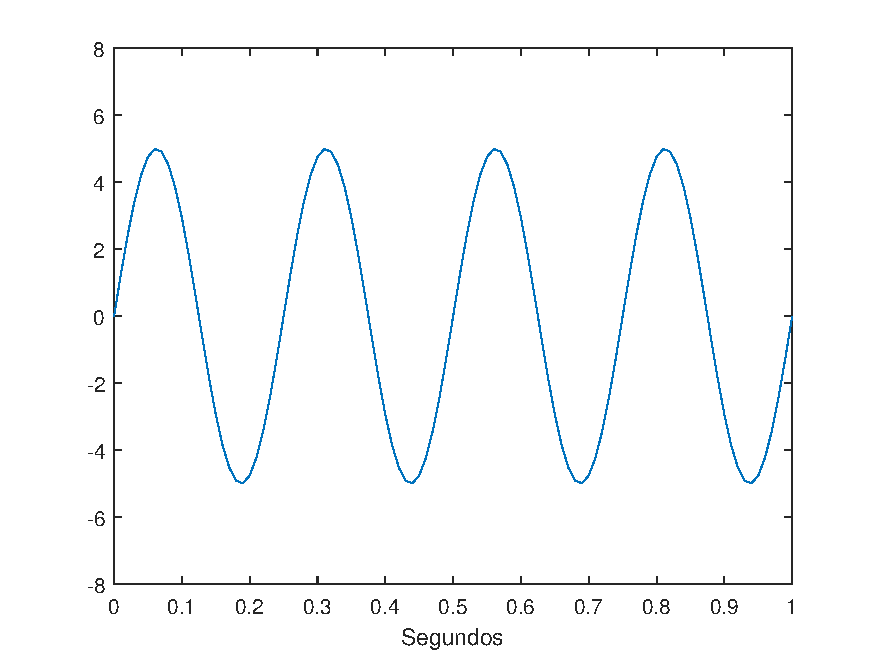
\includegraphics[width=0.75\textwidth]{onda sinusoidal.pdf}
\caption{Onda sinusoidal.}
\label{fig:onda sinusoidal}
\end{figure}

\newpage

Se definirmos a taxa de amostragem (\emph{sampling rate}) como sendo igual a 256 e a duração da amostragem (\emph{sampling duration}) como sendo igual a 1, podemos definir a variável dt como sendo o quociente entre a \emph{sampling duration} e o \emph{sampling rate}. E se representarmos a figura com pontos, podemos verificar que por cada segundo, temos 256 pontos.

\begin{lstlisting}[style=Matlab-editor, basicstyle=\small, caption={Slide 3.}, label={lst: sampling rate}]
sampling_rate = 256;
sampling_duration = 1; 
dt = sampling_duration/sampling_rate;
t = 0:dt:1;
F = 4;
A = 5;
y = A * sin(2 * pi * F * t);
plot(t, y, 'o', 'MarkerSize',4);
xlabel('Segundos')
\end{lstlisting}
    
\begin{figure}[!ht]
\centering
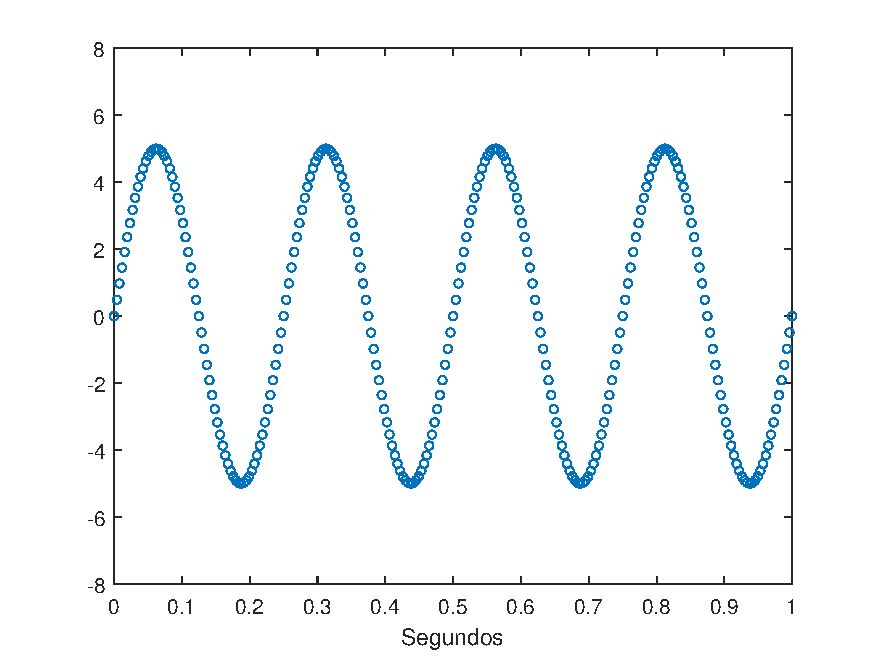
\includegraphics[width=0.75\textwidth]{samplingrate.pdf}
\caption{Taxa de amostragem.}
\label{fig:sampling rate}
\end{figure}

Agora uma função sinusoidal com frequência de 8~Hz e com uma determinada taxa de amostragem. Quando se altera o valor do passo de amostragem, para 8.5~Hz, obtêm-se um sinal com frequência de 0.5~Hz. Este exercicio, recriado em MATLAB no código da página seguinte, mostra a importância da escolha do passo de amostragem.

\newpage

\lstinputlisting[style=Matlab-editor, basicstyle=\small, caption={Slide 4.}, label={lst: undersampled}, firstline=2]{./codigo/undersampled.m}

\begin{figure}[!ht]
\centering
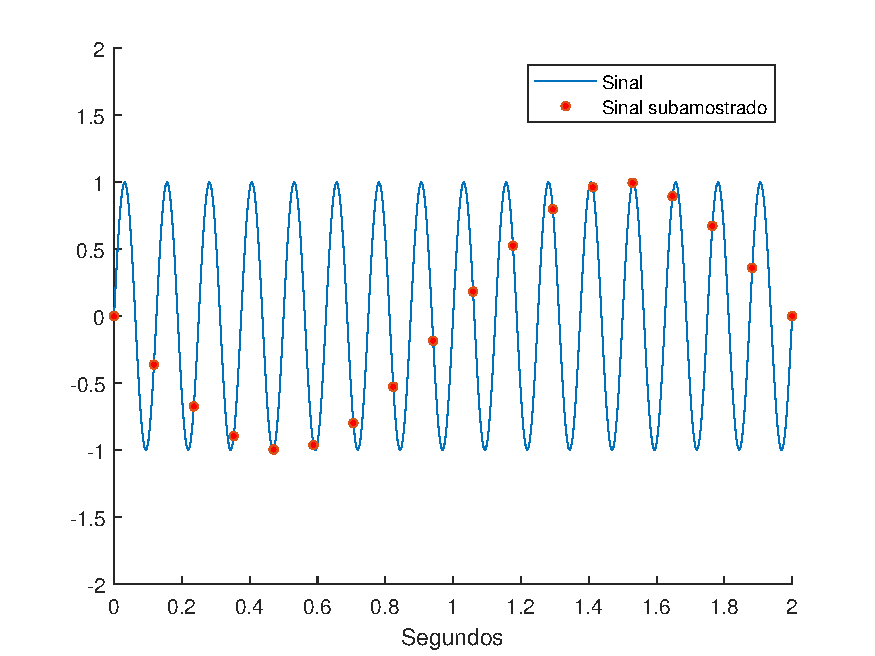
\includegraphics[width=0.75\textwidth]{undersampled.pdf}
\caption{Sinal subamostrado.}
\label{fig:undersampled}
\end{figure}